% Created by tikzDevice version 0.10.1 on 2016-08-22 16:25:48
% !TEX encoding = UTF-8 Unicode
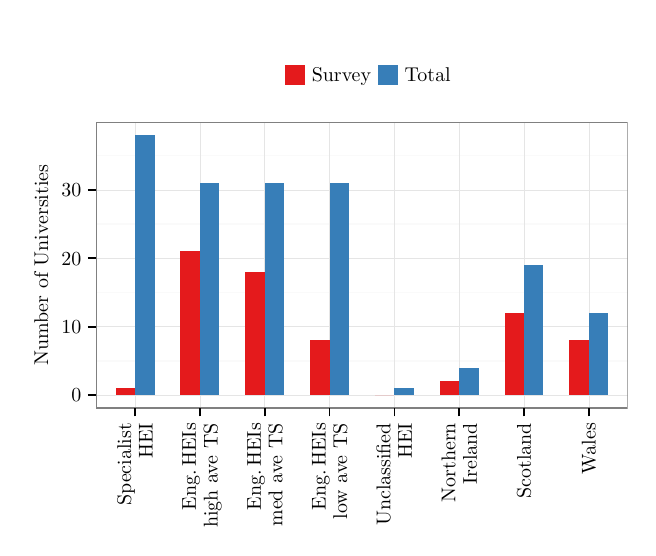
\begin{tikzpicture}[x=1pt,y=1pt]
\definecolor{fillColor}{RGB}{255,255,255}
\path[use as bounding box,fill=fillColor,fill opacity=0.00] (0,0) rectangle (216.81,180.67);
\begin{scope}
\path[clip] (  0.00,  0.00) rectangle (216.81,180.67);
\definecolor{drawColor}{RGB}{255,255,255}
\definecolor{fillColor}{RGB}{255,255,255}

\path[draw=drawColor,line width= 0.6pt,line join=round,line cap=round,fill=fillColor] (  0.00,  0.00) rectangle (216.81,180.68);
\end{scope}
\begin{scope}
\path[clip] ( 24.76, 43.19) rectangle (216.81,146.53);
\definecolor{fillColor}{RGB}{255,255,255}

\path[fill=fillColor] ( 24.76, 43.19) rectangle (216.81,146.53);
\definecolor{drawColor}{gray}{0.98}

\path[draw=drawColor,line width= 0.6pt,line join=round] ( 24.76, 60.25) --
	(216.81, 60.25);

\path[draw=drawColor,line width= 0.6pt,line join=round] ( 24.76, 84.97) --
	(216.81, 84.97);

\path[draw=drawColor,line width= 0.6pt,line join=round] ( 24.76,109.69) --
	(216.81,109.69);

\path[draw=drawColor,line width= 0.6pt,line join=round] ( 24.76,134.42) --
	(216.81,134.42);
\definecolor{drawColor}{gray}{0.90}

\path[draw=drawColor,line width= 0.2pt,line join=round] ( 24.76, 47.89) --
	(216.81, 47.89);

\path[draw=drawColor,line width= 0.2pt,line join=round] ( 24.76, 72.61) --
	(216.81, 72.61);

\path[draw=drawColor,line width= 0.2pt,line join=round] ( 24.76, 97.33) --
	(216.81, 97.33);

\path[draw=drawColor,line width= 0.2pt,line join=round] ( 24.76,122.06) --
	(216.81,122.06);

\path[draw=drawColor,line width= 0.2pt,line join=round] ( 38.81, 43.19) --
	( 38.81,146.53);

\path[draw=drawColor,line width= 0.2pt,line join=round] ( 62.23, 43.19) --
	( 62.23,146.53);

\path[draw=drawColor,line width= 0.2pt,line join=round] ( 85.65, 43.19) --
	( 85.65,146.53);

\path[draw=drawColor,line width= 0.2pt,line join=round] (109.07, 43.19) --
	(109.07,146.53);

\path[draw=drawColor,line width= 0.2pt,line join=round] (132.49, 43.19) --
	(132.49,146.53);

\path[draw=drawColor,line width= 0.2pt,line join=round] (155.92, 43.19) --
	(155.92,146.53);

\path[draw=drawColor,line width= 0.2pt,line join=round] (179.34, 43.19) --
	(179.34,146.53);

\path[draw=drawColor,line width= 0.2pt,line join=round] (202.76, 43.19) --
	(202.76,146.53);
\definecolor{fillColor}{RGB}{228,26,28}

\path[fill=fillColor] ( 31.78, 47.89) rectangle ( 38.81, 50.36);
\definecolor{fillColor}{RGB}{55,126,184}

\path[fill=fillColor] ( 38.81, 47.89) rectangle ( 45.84,141.83);
\definecolor{fillColor}{RGB}{228,26,28}

\path[fill=fillColor] ( 55.20, 47.89) rectangle ( 62.23, 99.81);
\definecolor{fillColor}{RGB}{55,126,184}

\path[fill=fillColor] ( 62.23, 47.89) rectangle ( 69.26,124.53);
\definecolor{fillColor}{RGB}{228,26,28}

\path[fill=fillColor] ( 78.63, 47.89) rectangle ( 85.65, 92.39);
\definecolor{fillColor}{RGB}{55,126,184}

\path[fill=fillColor] ( 85.65, 47.89) rectangle ( 92.68,124.53);
\definecolor{fillColor}{RGB}{228,26,28}

\path[fill=fillColor] (102.05, 47.89) rectangle (109.07, 67.67);
\definecolor{fillColor}{RGB}{55,126,184}

\path[fill=fillColor] (109.07, 47.89) rectangle (116.10,124.53);
\definecolor{fillColor}{RGB}{228,26,28}

\path[fill=fillColor] (125.47, 47.89) rectangle (132.49, 47.89);
\definecolor{fillColor}{RGB}{55,126,184}

\path[fill=fillColor] (132.49, 47.89) rectangle (139.52, 50.36);
\definecolor{fillColor}{RGB}{228,26,28}

\path[fill=fillColor] (148.89, 47.89) rectangle (155.92, 52.83);
\definecolor{fillColor}{RGB}{55,126,184}

\path[fill=fillColor] (155.92, 47.89) rectangle (162.94, 57.78);
\definecolor{fillColor}{RGB}{228,26,28}

\path[fill=fillColor] (172.31, 47.89) rectangle (179.34, 77.56);
\definecolor{fillColor}{RGB}{55,126,184}

\path[fill=fillColor] (179.34, 47.89) rectangle (186.36, 94.86);
\definecolor{fillColor}{RGB}{228,26,28}

\path[fill=fillColor] (195.73, 47.89) rectangle (202.76, 67.67);
\definecolor{fillColor}{RGB}{55,126,184}

\path[fill=fillColor] (202.76, 47.89) rectangle (209.78, 77.56);
\definecolor{drawColor}{gray}{0.50}

\path[draw=drawColor,line width= 0.6pt,line join=round,line cap=round] ( 24.76, 43.19) rectangle (216.81,146.53);
\end{scope}
\begin{scope}
\path[clip] (  0.00,  0.00) rectangle (216.81,180.67);
\definecolor{drawColor}{RGB}{0,0,0}

\node[text=drawColor,anchor=base east,inner sep=0pt, outer sep=0pt, scale=  0.72] at ( 19.36, 45.41) {0};

\node[text=drawColor,anchor=base east,inner sep=0pt, outer sep=0pt, scale=  0.72] at ( 19.36, 70.13) {10};

\node[text=drawColor,anchor=base east,inner sep=0pt, outer sep=0pt, scale=  0.72] at ( 19.36, 94.85) {20};

\node[text=drawColor,anchor=base east,inner sep=0pt, outer sep=0pt, scale=  0.72] at ( 19.36,119.58) {30};
\end{scope}
\begin{scope}
\path[clip] (  0.00,  0.00) rectangle (216.81,180.67);
\definecolor{drawColor}{RGB}{0,0,0}

\path[draw=drawColor,line width= 0.6pt,line join=round] ( 21.76, 47.89) --
	( 24.76, 47.89);

\path[draw=drawColor,line width= 0.6pt,line join=round] ( 21.76, 72.61) --
	( 24.76, 72.61);

\path[draw=drawColor,line width= 0.6pt,line join=round] ( 21.76, 97.33) --
	( 24.76, 97.33);

\path[draw=drawColor,line width= 0.6pt,line join=round] ( 21.76,122.06) --
	( 24.76,122.06);
\end{scope}
\begin{scope}
\path[clip] (  0.00,  0.00) rectangle (216.81,180.67);
\definecolor{drawColor}{RGB}{0,0,0}

\path[draw=drawColor,line width= 0.6pt,line join=round] ( 38.81, 40.19) --
	( 38.81, 43.19);

\path[draw=drawColor,line width= 0.6pt,line join=round] ( 62.23, 40.19) --
	( 62.23, 43.19);

\path[draw=drawColor,line width= 0.6pt,line join=round] ( 85.65, 40.19) --
	( 85.65, 43.19);

\path[draw=drawColor,line width= 0.6pt,line join=round] (109.07, 40.19) --
	(109.07, 43.19);

\path[draw=drawColor,line width= 0.6pt,line join=round] (132.49, 40.19) --
	(132.49, 43.19);

\path[draw=drawColor,line width= 0.6pt,line join=round] (155.92, 40.19) --
	(155.92, 43.19);

\path[draw=drawColor,line width= 0.6pt,line join=round] (179.34, 40.19) --
	(179.34, 43.19);

\path[draw=drawColor,line width= 0.6pt,line join=round] (202.76, 40.19) --
	(202.76, 43.19);
\end{scope}
\begin{scope}
\path[clip] (  0.00,  0.00) rectangle (216.81,180.67);
\definecolor{drawColor}{RGB}{0,0,0}

\node[text=drawColor,rotate= 90.00,anchor=base east,inner sep=0pt, outer sep=0pt, scale=  0.72] at ( 37.40, 37.79) {Specialist};

\node[text=drawColor,rotate= 90.00,anchor=base east,inner sep=0pt, outer sep=0pt, scale=  0.72] at ( 45.18, 37.79) {HEI};

\node[text=drawColor,rotate= 90.00,anchor=base east,inner sep=0pt, outer sep=0pt, scale=  0.72] at ( 60.82, 37.79) {Eng.\,HEIs};

\node[text=drawColor,rotate= 90.00,anchor=base east,inner sep=0pt, outer sep=0pt, scale=  0.72] at ( 68.60, 37.79) {high ave TS};

\node[text=drawColor,rotate= 90.00,anchor=base east,inner sep=0pt, outer sep=0pt, scale=  0.72] at ( 84.24, 37.79) {Eng.\,HEIs};

\node[text=drawColor,rotate= 90.00,anchor=base east,inner sep=0pt, outer sep=0pt, scale=  0.72] at ( 92.02, 37.79) {med ave TS};

\node[text=drawColor,rotate= 90.00,anchor=base east,inner sep=0pt, outer sep=0pt, scale=  0.72] at (107.66, 37.79) {Eng.\,HEIs};

\node[text=drawColor,rotate= 90.00,anchor=base east,inner sep=0pt, outer sep=0pt, scale=  0.72] at (115.44, 37.79) {low ave TS};

\node[text=drawColor,rotate= 90.00,anchor=base east,inner sep=0pt, outer sep=0pt, scale=  0.72] at (131.09, 37.79) {Unclassified};

\node[text=drawColor,rotate= 90.00,anchor=base east,inner sep=0pt, outer sep=0pt, scale=  0.72] at (138.86, 37.79) {HEI};

\node[text=drawColor,rotate= 90.00,anchor=base east,inner sep=0pt, outer sep=0pt, scale=  0.72] at (154.51, 37.79) {Northern};

\node[text=drawColor,rotate= 90.00,anchor=base east,inner sep=0pt, outer sep=0pt, scale=  0.72] at (162.28, 37.79) {Ireland};

\node[text=drawColor,rotate= 90.00,anchor=base east,inner sep=0pt, outer sep=0pt, scale=  0.72] at (181.82, 37.79) {Scotland};

\node[text=drawColor,rotate= 90.00,anchor=base east,inner sep=0pt, outer sep=0pt, scale=  0.72] at (205.24, 37.79) {Wales};
\end{scope}
\begin{scope}
\path[clip] (  0.00,  0.00) rectangle (216.81,180.67);
\definecolor{drawColor}{RGB}{0,0,0}

\node[text=drawColor,rotate= 90.00,anchor=base,inner sep=0pt, outer sep=0pt, scale=  0.72] at (  7.36, 94.86) {Number of Universities};
\end{scope}
\begin{scope}
\path[clip] (  0.00,  0.00) rectangle (216.81,180.67);
\definecolor{fillColor}{RGB}{255,255,255}

\path[fill=fillColor] ( 84.46,155.07) rectangle (157.11,172.14);
\end{scope}
\begin{scope}
\path[clip] (  0.00,  0.00) rectangle (216.81,180.67);
\definecolor{fillColor}{RGB}{228,26,28}

\path[fill=fillColor] ( 93.05,160.05) rectangle (100.16,167.16);
\end{scope}
\begin{scope}
\path[clip] (  0.00,  0.00) rectangle (216.81,180.67);
\definecolor{fillColor}{RGB}{55,126,184}

\path[fill=fillColor] (126.61,160.05) rectangle (133.73,167.16);
\end{scope}
\begin{scope}
\path[clip] (  0.00,  0.00) rectangle (216.81,180.67);
\definecolor{drawColor}{RGB}{0,0,0}

\node[text=drawColor,anchor=base west,inner sep=0pt, outer sep=0pt, scale=  0.72] at (102.68,161.12) {Survey};
\end{scope}
\begin{scope}
\path[clip] (  0.00,  0.00) rectangle (216.81,180.67);
\definecolor{drawColor}{RGB}{0,0,0}

\node[text=drawColor,anchor=base west,inner sep=0pt, outer sep=0pt, scale=  0.72] at (136.25,161.12) {Total};
\end{scope}
\end{tikzpicture}
